\newpage
\section{Aufgabenstellung 1 Taucher}

%% Gruppengröße die bereits geformten Teams
%% Alle verwendeten Quellen sind anzugeben.
%% Abzugeben bis zum 04.05.2025 um 23:59 Uhr
%% Abgabe = ein PDF-Dokument der gesamten Gruppe in folgendem Schema
                      
%%   SS2025_DevOps_ILV_Gruppe_[Gruppenbuchstabe]_Aufgabe_1 beispielsweise
%%   240223_DevOps_ILV_Gruppe_A_Aufgabe_1 für die Gruppe A

%% Bei Fragen kontaktiert mich gerne per E-Mail: stefan.taucher@fh-burgenland.at
%% Aufgabenstellung siehe Datei  Aufgabe.pdf .

\subsection{Teilbereich Build and Code}
Die Agile Softwareentwicklung in der Art und Weise wie Sie heute praktiziert und rezitiert wird, basiert auf 
dem Manifest für Agile Softwareentwicklung. Dieses ist die Basis für agiles Projektmanagement und wurde
2001 als Manifesto for Agile Software Development veröffentlicht. Dieses Manifest besteht aus vier Prinzipien:
\begin{itemize}
    \item Menschen und ihre Interaktion miteinander statt Prozesse und Werkzeuge.
    \item Funktionierende Produkte oder Dienstleistungen statt umfassender Dokumentation.
    \item Zusammenarbeit mit Kunden statt Vertragsverhandlungen.
    \item Reagieren auf Veränderungen statt Befolgen eines Plans. \cite{agile-manifesto}
\end{itemize} 
  
Es lässt sich also sagen, dass Agile Software Entwicklung sich aus an Agilität ausgerichteten
Methoden und agilen Prozessen zusammensetzt. 

% Please add the following required packages to your document preamble:
% \usepackage{graphicx}
\subsubsection{Vorgehensmodelle}
\textbf{Fragestellung:} \textit{Welche bereits vorgestellten bzw. zusätzlich recherchierte Vorgehensmodelle ermöglichen ein
schnelles Iterieren und somit die Möglichkeit Feedback zeitnah durch die jeweiligen Stakeholder
einzubringen? Zusätzlich soll auch darauf eingegangen werden, weshalb die gewählten
Vorgehensmodelle dies im Vergleich zu anderen Modellen ermöglichen.}
\\

Aufbauend auf das agile Manifest haben sich eine Vielzahl von Frameworks, für das Management der agilen Prozesse entwickelt. 
Diese sind mit Fokus auf die Software Entwicklung entstanden, haben aber ihren Weg auch schon in andere Bereiche angetreten. 
Einige ausgewählte Frameworks sollen nachfolgenden kurz präsentiert werden. 
\newline
\begin{table}[h!]
    \centering
    \caption{Agile Prozessmanagement Frameworks der Software Entwicklung}
    \label{tab:agile-frameworks}
    \begin{tabular}{|l|l|}
    \hline
    \textbf{Framework}            & \textbf{Abkürzung} \\ \hline
    Extreme Programming           & XP                 \\ \hline
    Feature Driven Development    & FDD                \\ \hline
    Kanban in der IT              & IT-Kanban          \\ \hline
    Adaptive Software Development & ASD                \\ \hline
    Crystal Family                & CF                 \\ \hline
    Agile unified process         & AUP                \\ \hline
    Lean software development     & LSD                \\ \hline
    Large Scale Agile Frameworks  & LSAF               \\ \hline
    \end{tabular}
\end{table} 
\newline
Die Leitwerte des \textbf{XP} sind Kommunikation, Einfachheit, Feedback und Mut und sollen durch die Praktiken:
Vor-Ort-Kunde, Planspiel, Metapher, einfaches Design, kleines Release, Pair Programming, Testen, Refactoring, 
kontinuierliche Integration, 40-Stunden-Woche, Coding Standard und kollektive Verantwortung für die Entstehung 
eines optimalen Produktes sorgen. Einige dieser Praktiken bzw. Methoden werden auch in anderen agilen Frameworks 
genutzt, im XP wird aber stark auf die Synergieeffekte zwischen den Leitwerten und Praktiken wert gelegt. \cite{FOJTIK20111464}
\newline Mohammad Alshayeb und Wie Li untersuchten die spezifischen Praktiken und stellten im XP folgende Tätigkeiten
als Hauptaktivitäten der Entwickler fest: Refactoring, neues Design, Beheben von Fehlern und Implementieren von Unit- 
sowie Funktionstests, um die Funktionstüchtigkeit des Produktes sicherzustellen. \cite{Alshayeb2006-nt} \\

Das \textbf{FDD} hat sich aus der Coad Methode von Peter Coad entwickelt und besteht lediglich aus zwei Hauptphasen. 
Der Entdeckungs- und der Implementierungsphase. Hauptaugenmerk wird dabei auf die Entdeckungsphase gelegt, da hier sowohl die 
Liste der Features erstellt wird, als auch die UML-Diagramme der spezifischen Kundendomäne. 
Die Mitwirkung des Kunden ist besonders wichtig, damit die Wartbarkeit und Erweiterbarkeit des Codes im weiteren Projektverlauf gewährleistet werden kann. 
Die verwendete Sprache sollte von sowohl von Entwickler:innen, als auch von Kundenseite verstanden werden. \cite{Chowdhury2011-hg} \\

\textbf{Kanban} ist eine Methodik aus der Produktionsindustrie und wurde von Mary und Tom Poppenieck, und später von David Anderson für 
die Software Entwicklung adaptiert. Im Gegensatz zu den meisten anderen agilen Frameworks gibt es keine spezifischen Arbeitsabläufe, 
Rollen oder zeitliche Begrenzungen des Arbeitsprozesses in Iterationen. 
Hauptaufgabe ist es, den Arbeitsfluss zu koordinieren und in Teilaufgaben zu unterteilen. Anderson beschreibt dazu fünf Kernprinzipien für IT-Kanban:

\begin{itemize}
    \item Arbeitsablauf visualisieren
    \item Arbeit, die noch nicht abgeschlossen ist, begrenzen des Work in Progress
    \item Arbeitsfluss messen und verwalten
    \item Richtlinien für den Arbeitsprozess definieren und explizit sichtbar machen
    \item Nutzung von Modellen aus Praxis oder Theorie, um Verbesserungsmöglichkeiten im Arbeitsablauf zu erkennen.
\end{itemize}

Die Visualisierung erfolgt durch das sogenannte Kanban-Board, das sowohl die Begrenzung der Arbeitslast bzw. des Arbeitspakets, 
als auch die Priorisierung der Aufgabe und das Eingreifen bei Engpässen im Arbeitsfluss ermöglicht. \\
\cite{Ahmad2018-jv,Granulo2019-wm} \\

In \textbf{ASD} wird der Fokus auf ein zyklisches Weiterentwicklungsmodell gelegt, das die unterschiedlichen Phasen im Lebenszyklus
der Software widerspiegelt. \cite{Abdelaziz2015-lb}
\begin{figure}[h!]
\centering
\caption{ASD-Diagramm}
    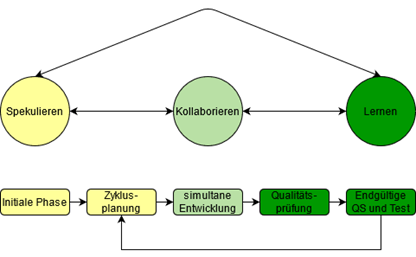
\includegraphics[width=0.8\textwidth]{fig/ASD.png}
    \label{fig:ASD-diagram}
\end{figure}
\begin{itemize}
    \item \textbf{Spekulieren:} Ersetzt planen, um hier mehr Raum für Innovation und Ungewissheit bei komplexen Problemen zu schaffen.
    \item \textbf{Kollaborieren/Zusammenarbeiten:} Bei komplexen Software-Anwendungen und sich ändernden Anforderungen ist der Informationsfluss nur durch die Zusammenarbeit im Team schaffbar.
    \item \textbf{Lernen:} In dieser Phase können die technischen Parameter und Kundenwünsche regelmäßig nach den abgeschlossenen einzelnen Iterationen überprüft werden
\end{itemize}
\cite{Alnoukari2008-ro,Abdelaziz2015-lb} \\

Die \textbf{CF} wurde von Alistair Cockburn erstellt, um im Rahmen der Entwicklung von Software, ähnlich wie bei einem Kristall oder Edelstein, 
je nach Größe des Projektes unterschiedliche Methoden, Techniken und Richtlinien nutzen zu können. Die Methoden fokussieren sich 
dabei auf folgende Parameter \cite{Ibrahim2020-ip}:
\begin{itemize}
    \item \textbf{Menschen}
    \item \textbf{Interaktionen} 
    \item \textbf{Gemeinschaft}    
    \item \textbf{Fertigkeiten}
    \item \textbf{Talente und Kommunikation }
\end{itemize}
Die Methoden von Crystal werden nach Farben benannt und nach der Größe des Projektes und der Anzahl der Projektmitarbeiter*Innen eingeteilt.
\begin{figure}[h!]
    \centering
    \caption{CS-Diagramm}
        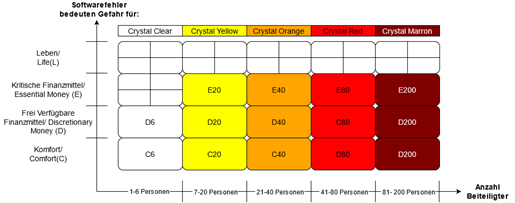
\includegraphics[width=1\textwidth]{fig/CSD.png}
        \label{fig:CS-diagram}
    \end{figure}
Auf der Y-Achse werden die vier Level des Gefahrenlevels definiert und auf der X-Achse die Anzahl der Beteiligten. 
Hier angezeigt werden die Crystal Methoden, die noch nicht das Risikolevel Leben abdecken können. 
Crystal Clear sollen Projekte mit fixiertem Preis und klaren Parameter sein und sobald Projekte Gefahr für Leib 
und Leben beinhalten, handelt es sich dabei um Crystal Diamond und Crystal Sapphire.\cite{cockburn2004,Ibrahim2020-ip} \\

\textbf{AUP} ist ein Framework bzw. Modellierungsansatz, der von Scott Ambler aus dem Rational Unified Process (RUP) mit agilen Methoden kombiniert entwickelt wurde. 
Ambler definiert dafür folgende Kernprinzipen \cite{Christou2010-vf}:
\begin{itemize}
    \item Die meisten Menschen werden keine detaillierte Dokumentation lesen.  Sie werden jedoch hin und wieder Anleitung und Schulung benötigen
    \item Das Projekt sollte einfach mit wenigen Seiten beschrieben werden.
    \item Die AUP entspricht den von der Agile Alliance beschriebenen Werten und Prinzipien.    
    \item Das Projekt muss sich darauf konzentrieren, einen wesentlichen Wert zu liefern und nicht unnötige Funktionen.
    \item Die Entwickler müssen die Freiheit haben, Werkzeuge zu verwenden, die für die jewei-lige Aufgabe am besten geeignet sind, und nicht, um eine Vorschrift zu erfüllen.
    \item AUP lässt sich über gängige HTML-Editierwerkzeuge leicht anpassen. 
\end{itemize}
Es werden dann vier seriell ablaufende Phasen definiert \cite{Li2010-ge,ShuiYuan2009-or}:
\begin{itemize}
    \item \textbf{Inception/Beginn}: Ziel ist es, den anfänglichen Umfang des Projekts und eine potenzielle Architektur für Ihr System festzulegen, sowie die anfängliche Projektfinanzierung und die Akzeptanz der Stakeholder zu erhalten.
    \item \textbf{Elaboration/Ausarbeitung:} Die Architektur des Systems wird überprüft.
    \item \textbf{Construction/Konstruktion: }Es soll regelmäßig und schrittweise funktionierende Software erstellt werden, welche die Anforderungen der Projektbeteiligten mit höchster Priorität erfüllt.
    \item \textbf{Transition/Übergabe:} Das Ziel ist die Validierung und der Einsatz ihres Systems in ihrer Produktionsumgebung
\end{itemize}

LSD hat als Vorbild das Toyota Produktionssystem und definiert sieben Prinzipien und 22 Praktiken für die Umsetzung im Rahmen der agilen Softwareentwicklung. 
Die sieben Prinzipien sind \cite{Janes2015-ir,Jonsson2013-gn}:
\begin{itemize}
    \item Verschwendung vermeiden
    \item Lernen unterstützen
    \item So spät entscheiden wie möglich
    \item Verantwortung an das Team geben
    \item Integrität einbauen
    \item Das Ganze sehen
\end{itemize}
Unterschiedliche \textbf{LSAF}  sind entwickelt worden, um agile Praktiken auf große Projekte und Softwareentwicklung 
mit weltweit verteilten Teams anzuwenden. Zu den bekanntesten Modellen zählen\cite{Beecham2021-jj,Ebert2017-jz}:
\begin{itemize}
    \item \textbf{Scrum of Scrums (SoS)}
    \item \textbf{Scaled Agile Framework (SAFe)} 
    \item \textbf{Large-Scale Scrum (LeSS)}    
    \item \textbf{Disciplined Agile Delivery (DAD)}
    \item \textbf{Lean Scalable Agility for Engineering (LeanSAFE)}
\end{itemize}
Kieran Conboy und Noel Carroll definieren ausgehend von einer 15-jährigen Retrospektive folgende Herausforderungen bei der
Implementation von Large Scale Agile Frameworks \cite{Conboy2019-uw,Kasauli2021-jn}:
\begin{itemize}
    \item Definieren von Konzepten
    \item Vergleich und Gegenüberstellung von Frameworks
    \item Bereitschaft und Appetit auf Veränderung
    \item Abgleich von Organisationsstruktur und Rahmenbedingungen
    \item Top-down- versus Bottom-up-Implementierung
    \item Überbetonung der 100 \%igen Einhaltung der Regeln des Frameworks gegenüber dem Mehrwert für die Firma
    \item Fehlender evidenzbasierter Einsatz
    \item Erhaltung der Autonomie der Entwickler und Entwicklerteams
    \item Fehlende Abstimmung zwischen Kundenprozessen und Frameworks
\end{itemize}

\subsubsection{Agile Methoden und Praktiken}
Es existiert eine große Vielfalt an unterschiedlichen Methoden. Zur Vereinfachung werden diese kurz in Englisch angeführt:
\begin{table}[h!]
    \centering
    \caption{Tabellarische Auflistung agiler Methoden}
    \label{tab:agile-methods}
    \begin{tabular}{|l|l|}
    \hline
    \textbf{Methoden} & \textbf{Abkürzung} \\ \hline
    Acceptance test-driven development  & ATDD                 \\ \hline
    Agile modeling    & AM                \\ \hline
    Agile testing             & AT          \\ \hline
    Backlogs & BL                \\ \hline
    Behavior-driven development & BDD                 \\ \hline
    Cross-Functional Team     & DST                \\ \hline
    Daily Stand-up    & CFT                \\ \hline
    Domain-driven design   & DDD               \\ \hline
    Iterative and incremental development    & IID               \\ \hline
    Planning poker  & PlP               \\ \hline
    Refactoring  & RF               \\ \hline
    Retrospective  & RS               \\ \hline
    Specification by example  & SBE               \\ \hline
    Story-driven modeling  & SDM               \\ \hline
    Timeboxing   & TB               \\ \hline
    Velocity tracking   & VT               \\ \hline
    \end{tabular}
\end{table} \\

\textbf{ATTD:} Hierbei handelt es sich um eine Methode, welche großen Wert auf die Kommunikation der Kund*Innen, Entwickler*Innen und Tester*Innen legt. 
Wichtig sind hierbei die Implementierung von Akzeptanztests bevor die Entwicklungsteams mit dem Programmieren beginnen.
Diese Tests sollen in der Sprache der Geschäftsdomäne geschrieben werden. Eine Anforderung bzw.
User Story für welche kein Test vor Anforderungsumsetzung geschrieben wurde, ist schlecht implementiert.\cite{Downs2011-uk}\\

\textbf{AM:} Dies ist eine Methode für Modellierung und Dokumentation von Softwaresystemen,
die auf unterschiedlichen Kernprinzipien beruht.\cite{Ambler2010-te} \\

\textbf{AT:} Hiermit werden die Parameter für das Testen und Testszenarien im agilen Softwareentwicklungsumfeld beschrieben.
Der Fokus liegt auf der Unterstützung der Entwicklungsteams.  Ein Beispiel für die Implementierung ist die Definition Of Test (DoT),
die die Parameter für die Testdurchführung und Strategie definiert. \cite{Crispin2009} \\

\textbf{BL} sind eine Liste von Arbeitspaketen, die geordnet sind nach Priorität und Reifegrad der einzelnen Artefakte.
Die bekanntesten Varianten der Arbeitspaketformate sind User Stories oder Use Cases.
Es werden Features, Problemlösungen und andere nicht technische Anforderungen dokumentiert,
um ein Softwareprodukt liefern zu können.\cite{Svensson2019-pq} \\

\textbf{BDD} ist eine agile Testtechnik, deren Ziel es ist, Software-Anforderungen als Beispielinteraktionen mit dem System zu spezifizieren,
wobei eine strukturierte natürliche Sprache verwendet wird. Während die Beispiele (in der Theorie)
von nicht-technischen Stakeholdern gelesen werden können, können sie auch gegen die Codebasis ausgeführt werden,
um Verhaltensweisen zu identifizieren, die noch nicht korrekt implementiert sind. \cite{Binamungu2020-wt} \\

\textbf{CFT:} Hierbei handelt es sich um Teams aus unterschiedlichen Fachbereichen einer Firma.
Ziel ist es, die Wissenssilos innerhalb der eigenen Organisation aufzubrechen und damit die Kundenbe-dürfnisse an die erste Stelle zu bringen.
Innerhalb der Softwareentwicklung bedeutet dies oft, dass Frontend, Backend, Devops, Tester*Innen,
Interface Designer*Innen und Personen, die für die Geschäftslogik zuständig sind, zusammenarbeiten. \cite{McDonough2000-fi} \\

\textbf{DST:} Dies ist eine spezifische Meeting-Art, die täglich stattfinden soll,
um sich gegenseitig über den aktuellen Stand der Arbeit zu informieren.
Diese Meetings sollten time-boxed (siehe weiter unten) sowie im Stehen stattfinden,
um das Meeting fokussiert durchzuführen. Je nach Umsetzung gibt es dafür einen kurzen Fragenkatalog. \cite{Stray2016-me} \\

\textbf{DDD} ist eine Vorgehensweise, in der versucht wird, das Domänenwissen für den Softwareentwurf korrekt abzufragen,
zu erfassen und modellbasiert darzustellen. Ziel ist, die Beziehungen unterschiedlicher Domänenkonzepte zu identifizieren.
DDD findet oft Anwendung beim Entwurf von Microservice-Architekturen,
da es eine Schnittmenge zwischen den einzelnen funktionalen Microservices und den verschiedenen Geschäftsfeldern gibt. \cite{Rademacher2018-yo} \\

\textbf{IID} ist die Sammelbezeichnung für unterschiedliche Konzepte und Modelle für iterative und inkrementelle Vorgehensmodelle
in der Softwareentwicklung. Diese verschiedenen Ansätze sind aber alle der Versuch eines Gegenmodelles zum traditionellen Ansatz einer
gleichzeitigen In-tegration aller Teilkomponenten zum Abschluss des Projektes.
Durch kleine, häufige Schritte und Auslieferung von Teilsystemen, soll eine sequenzielle,
dokumentengesteuerte Auslieferung in einem Durchgang vermieden werden. \cite{Larman2003-fg} \\

\textbf{PlP}  ist Teil der Planungsmeetings für die nächste Iteration und dient der Schätzung der Zeitres-sourcen,
die notwendig sind, um ein neues Feature zu implementieren.
Die Kalkulation erfolgt zumeist in sogenannten Story Points, die in der Regel einem idealen Arbeitstag entsprechen. 
Zumeist werden für die Schätzung vordefinierte Werte wie die Fibonacci-Folge verwendet. \\
\cite{Mahnic2012-ve} \\

\textbf{RF} ist der Prozess, in dem der Quellcode so umstrukturiert wird, dass die interne Codequalität und Struktur
der Software verbessert wird, dabei aber das externe Verhalten, das für die Benutzer ersichtlich ist, gleichbleibt.
Ziel ist es, die Wartungskosten zu verringern und die Lebensdauer der Software zu verlängern. \cite{Kaur2019-wy} \\

\textbf{RS} sind Meetings bzw. Aktivitäten zur Erfahrungssicherung der Teammitglieder. 
Oft auch als Post-Mortems bezeichnet, in der die Probleme sowie Ursachen eines abgeschlossenen Projektes oder einer Softwareiteration analysiert werden. 
Es sollen durch diese Untersuchung sowohl die Erfolgsfaktoren als auch die Auslöser von Problemen erkannt werden. \cite{Lehtinen2014-ou} \\

\textbf{SBE} ist ein Leitfaden oder eine kollaborative Methode, deren oberstes Ziel die Entwicklung von Software ist,
welche die Kundenanforderungen erfüllt. Es wird hier mit Workshops gearbeitet, in denen die verschiedenen Rollen und Standpunkte
vertreten sind und die gemeinsam spezifischen Szenarien der Nutzung anhand von Beispielen entwerfen.
Mit Hilfe dieser Szenarien sollen fol-gend die automatisierten und funktionalen Tests entwickelt werden. Ziel ist es, eine Dokumentation zu erstellen, 
die in der Sprache der jeweiligen Fachdomäne geschrieben wurde und auch von Personen aus den Fachabteilungen,
die keine Programmierer sind, gelesen werden kann. \cite{Blasquez2017-og,Bache2014-cp} \\

Im Gegensatz zu anderen Arten der objektorientierten Modellierung wird im \textbf{SDM}
die Struktur nicht durch statische Klassendiagramme und der Beziehung dieser Klassen zueinander Wert gelegt,
sondern auf die Erstellung von spezifischen Beispielen, die Szenarien in der Nutzung abbilden.
Zudem sollen die daraus entstehenden Objektdiagramme sich im Laufe des Szenarios und der Ausführung
der Software weiterentwickeln. \cite{Wautelet2017-rv} \\

\textbf{TB} ist die Definition eines Zeitrahmens oder einer Zeitphase,
die innerhalb der Projektplanung für gewisse Vorgänge genutzt werden darf. Es wird hier ein Zeitbudget für die jeweiligen Aufgaben erstellt.
Insbesondere im Scrum und der agilen Softwareentwicklung wird Timeboxing für
einzelne Vorgänge wie Meetings und Iterationszyklen verwendet. \cite{Miranda2011-yh} \\

\textbf{VT} ist die Messung und Darstellung der Team Performanz. Zwei für die Darstellung verwendete Methoden
sind Burn-Down und Burn-Up Charts. \\
\cite{Al-Sabbagh2018-bd} \\

Bei diesen verschiedenen Praktiken ist ersichtlich, dass einige bereits die Produktivität (z.B. IID, VT, PlP, BL),
Ergebnisorientierung (z.B.: RF, TB) sowie die Weiterentwicklung der Teams (z.B.: RF, PP, AT, AM) innerhalb der
agilen Softwareentwicklung mitgedacht bzw. angedacht haben.

\subsubsection{Extreme Programming}

\textbf{Fragestellung:} \textit{Beschreiben Sie mindestens 3 Praktiken aus Extreme Programming im Detail und den Einfluss
die diese Praktik auf die Softwareentwicklung und dem Ergebnis haben.}

\paragraph{Pair Programming}
Beim Pair Programming arbeiten zwei Entwickler gemeinsam an einem Computer. Eine Person (der Driver) schreibt den Code, 
während die andere Person (der Navigator) den Code überprüft, Probleme identifiziert und strategische Entscheidungen trifft. 
Die Rollen werden regelmäßig gewechselt. 

\textbf{Einfluss auf die Softwareentwicklung:}
\begin{itemize}
    \item \textbf{Verbesserte Codequalität:} Durch kontinuierliches Review werden Fehler früher erkannt und behoben.
    \item \textbf{Wissenstransfer:} Entwickler lernen voneinander, was zu einer breiteren Verteilung von Wissen im Team führt.
    \item \textbf{Bessere Lösungsansätze:} Durch die Kombination verschiedener Perspektiven entstehen oft kreativere und effizientere Lösungen.
    \item \textbf{Reduzierte technische Schulden:} Die kontinuierliche Überprüfung verhindert Abkürzungen und schlechte Praktiken.
\end{itemize}

\paragraph{Continuous Integration (CI)}
Bei der Continuous Integration werden Codeänderungen mehrmals täglich in ein gemeinsames Repository integriert. Nach jeder Integration 
werden automatisierte Tests durchgeführt, um sicherzustellen, dass die Änderungen keine Fehler verursachen.
\\

\textbf{Einfluss auf die Softwareentwicklung:}
\begin{itemize}
    \item \textbf{Frühe Fehlererkennung:} Probleme werden unmittelbar nach ihrer Entstehung identifiziert, was die Behebungskosten drastisch reduziert.
    \item \textbf{Reduzierte Integrationszeit:} Durch häufige kleine Integrationen werden große, problematische Merges vermieden.
    \item \textbf{Höhere Softwarestabilität:} Die Software bleibt kontinuierlich in einem funktionsfähigen Zustand.
    \item \textbf{Schnelleres Feedback:} Entwickler erhalten unmittelbare Rückmeldung zu ihren Änderungen.
\end{itemize}

\paragraph{Test-Driven Development (TDD)}
Bei TDD werden Tests geschrieben, bevor der eigentliche Code implementiert wird. Der Entwicklungsprozess folgt 
einem Red-Green-Refactor-Zyklus: Zuerst wird ein fehlschlagender Test geschrieben (Red), dann wird gerade genug Code implementiert,
um den Test zu bestehen (Green), und schließlich wird der Code verbessert, ohne seine Funktionalität zu ändern (Refactor).
\\

\textbf{Einfluss auf die Softwareentwicklung:}
\begin{itemize}
    \item \textbf{Klarere Anforderungen:} Das Schreiben von Tests zwingt Entwickler, die Anforderungen genau zu verstehen.
    \item \textbf{Besseres Design:} TDD fördert modularen, entkoppelten Code, der leichter zu testen ist.
    \item \textbf{Umfassende Testabdeckung:} Jede Funktionalität wird durch Tests abgedeckt, was zu robusterer Software führt.
    \item \textbf{Dokumentation durch Tests:} Tests dienen als lebende Dokumentation, die zeigt, wie der Code verwendet werden soll.
    \item \textbf{Sicherheit bei Refactoring:} Entwickler können Code mit Vertrauen umgestalten, da Tests Regressionen aufdecken.
\end{itemize}

    %% possibile quellens:


    %% https://www.it-agile.de/agiles-wissen/agile-entwicklung/was-ist-extreme-programming/
    %% https://www.agile-heroes.com/de/magazine/extreme-programming/
    %% https://asana.com/de/resources/extreme-programming-xp


\subsubsection{Zusammenfassung von Artikel Spotify Scaling}
\textbf{Aufgabenstellung:} \textit{Lesen Sie den Artikel https://blog.crisp.se/wp-content/ \\
uploads/2012/11/SpotifyScaling.pdf.
Diese Informationen fassen Sie bitte in 1 bis maximal 2 Seiten zusammen}

\paragraph{Das Spotify-Modell zur Skalierung agiler Organisationen:}
Das Spotify-Modell stellt eines der meistzitierten Beispiele für die Skalierung agiler Methoden in der zeitgenössischen Softwareentwicklung dar.
Es wurde 2012 von Kniberg und Ivarsson öffentlich vorgestellt. In einer Phase rapiden Wachstums mit Niederlassungen
in mehreren Städten entwickelte Spotify eine Organisationsstruktur, die darauf abzielte, Agilität durch kleine,
autonome Teams zu bewahren und gleichzeitig Kohärenz, Wissensaustausch und architektonische Integrität sicherzustellen.

\paragraph{1. Squads - Autonome Feature-Teams:}Ein Squad bei Spotify ist ein funktionsübergreifendes,
selbstorganisierendes Team mit einer langfristigen Mission (z.B. Android-Client, Backend-Skalierung, Zahlungssysteme).
Die Squads wählen ihre eigenen Arbeitsprozesse (Scrum, Kanban oder hybride Ansätze) und integrieren Lean-Startup-Prinzipien -
sie veröffentlichen MVPs (Minimum Viable Products) und nutzen Daten aus A/B-Tests,
um dem Motto \textit{Denken, Bauen, Ausliefern, Optimieren} zu folgen.
Um Innovation zu fördern, widmet jedes Squad etwa 10\% seiner Zeit sogenannten Hack Days.
In diesen Phasen verfolgen Teammitglieder Nebenprojekte oder experimentieren mit neuen Werkzeugen,
was häufig zu Verbesserungen bei Produkten oder Entwicklungswerkzeugen führt. Product Owner verantworten die Priorisierung des Backlogs,
während Agile Coaches (in die Squads integriert) Retrospektiven moderieren und die Weiterentwicklung der Arbeitsprozesse unterstützen.

\paragraph{2. Tribes - Kohärente Domänen:}
Thematisch zusammenhängende Squads bilden einen Tribe, dessen Größe typischerweise auf etwa 100 Personen begrenzt ist -
in Anlehnung an die Dunbar-Zahl, um informellen sozialen Zusammenhalt zu gewährleisten und Bürokratie zu minimieren.
Tribes veranstalten regelmäßige Demonstrationen, bei denen Squads ihre Fortschritte, Werkzeuge und Ergebnisse ihrer Hack-Days präsentieren.

\paragraph{Abhängigkeitsmanagement}
Spotify führt vierteljährliche Umfragen unter den Squads durch, um Abhängigkeiten zu erfassen und blockierende Probleme zu identifizieren. 
Diese werden als Kreise (aktueller Zustand) und Pfeile (Trend) visualisiert. Die erhobenen Daten führen zu Priorisierungsanpassungen,
Reorganisation oder architektonischen Veränderungen, um Engpässe zu beseitigen. Anstelle eines permanenten Scrum of Scrums findet
die Koordination zwischen Squads bedarfsorientiert statt - beispielsweise als temporäre tägliche Synchronisation mit einem gemeinsamen Board
für Notizen im Rahmen eines Squad-übergreifenden Projekts.

\paragraph{3. Chapters und Guilds - Horizontale Gemeinschaften:}
Um Silobildung zu vermeiden, führte Spotify Chapters (fachbereichsbezogene Gruppen innerhalb eines Tribes,
geleitet von einem Chapter Lead, der gleichzeitig als Linienmanager fungiert) und Guilds
(organisationsweite, freiwillige Interessengemeinschaften) ein. Chapters gewährleisten technische Konsistenz, während Guilds
(z.B. Web Guild Unconference) den Wissensaustausch und die Werkzeugentwicklung über Tribe-Grenzen hinweg ermöglichen,
vergleichbar mit Communities of Practice.

\paragraph{4. Architektur und Systemeigentümerschaft:}
Das Backend von Spotify besteht aus über 100 lose gekoppelten Diensten. Squads können diese unabhängig bereitstellen,
riskieren dabei jedoch \textit{Architekturerosion}. Um diesem Risiko entgegenzuwirken, verfügt jedes System über einen System Owner –
häufig ein Squad-Mitglied oder ein DevOps-Paar, das für Stabilität, Dokumentation, technische Schulden und periodische
\textit{System-Owner-Tage}  zur Systempflege verantwortlich ist. Ein Chief Architect bietet übergeordnete Leitlinien in beratender Funktion
und stellt sicher, dass neue Dienste mit der architektonischen Gesamtvision übereinstimmen, ohne die Autonomie der Squads zu untergraben.

\paragraph{5. Operations-Team als Ermöglicher:}
Anstelle eines Übergabemodells baut und pflegt ein Operations-Team bei Spotify die Release-Infrastruktur
(Skripte, Routinen, Umgebungen), damit Squads ihre Releases selbstständig durchführen können.
Diese \textit{Straße zur Produktion} reduziert Reibung zwischen Entwicklung und Betrieb und verkörpert DevOps-Ideale geteilter Verantwortung.

\paragraph{6. Implikationen für DevOps und skalierte Agilität:} Das Spotify-Modell veranschaulicht exemplarisch,
wie dezentralisierte Autonomie und leichtgewichtige Abstimmungsstrukturen koexistieren können. Es unterstreicht:

\begin{itemize}
    \item \textbf{Kontinuierliche Experimentation} durch MVPs, A/B-Tests und Hack Days
    \item \textbf{Dynamische Koordination} durch bedarfsgesteuerte Synchronisation und Abhängigkeitsanalysen
    \item \textbf{Gemeinsame Verantwortung} durch System Owners und ein unterstützendes Operations-Team
    \item \textbf{Wissensnetzwerke} ermöglicht durch Chapters und Guilds
\end{itemize}

Als Fallstudie illustriert es den iterativen, menschenzentrierten Ansatz, der erforderlich ist,
um Agilität in großen, schnell wachsenden Softwareorganisationen aufrechtzuerhalten.

\subsubsection{Git Features}

Fragestellung: Beschreiben Sie Git im Detail sowie mindestens 2 Features im Detail.

\paragraph{Was ist Git?}
Git ist ein verteiltes Versionskontrollsystem, das 2005 von Linus Torvalds entwickelt wurde.
Es ermöglicht die Verwaltung von Änderungen an Dateien und Projekten,
wobei jeder Entwickler eine vollständige Kopie des Projekts und seiner Historie auf seinem lokalen System hat.
Git ist besonders für seine Geschwindigkeit, Datenintegrität und Unterstützung für nicht-lineare, verteilte 
Workflows bekannt. \cite{github-git}

\paragraph{Feature 1: Branching und Merging}
Git bietet ein leistungsfähiges Branching-System, das es ermöglicht, parallele Entwicklungslinien 
zu erstellen und zu verwalten. Branches sind leichtgewichtige Zeiger auf einen bestimmten Commit. 
Entwickler können schnell neue Branches erstellen, zwischen ihnen wechseln und sie zusammenführen. 
Dies ermöglicht:

    \begin{itemize}
        \item Isolierte Entwicklung neuer Features
        \item Experimentieren ohne Risiko für den Hauptcode
        \item Parallele Arbeit an verschiedenen Aspekten des Projekts
        \item Einfaches Zusammenführen von Änderungen durch Merging
    \end{itemize}

    \paragraph{Feature 2: Distributed Version Control}
    Git ist ein vollständig verteiltes System, was bedeutet, dass jeder Entwickler eine vollständige Kopie des Repositories besitzt.
    Dies bietet mehrere Vorteile:

    \begin{itemize}
        \item Offline-Arbeit ist möglich
        \item Schnelle Operationen durch lokale Ausführung
        \item Redundanz und Backup durch multiple Kopien
        \item Flexible Workflow-Möglichkeiten
        \item Keine zentrale Schwachstelle
    \end{itemize}




    %% possibile quellens:
    %% https://docs.github.com/en/get-started/using-git/about-git
    %% https://www.geeksforgeeks.org/git-features/
    %% https://www.simplilearn.com/tutorials/git-tutorial/what-is-git#features_of_git


\subsubsection{Qualitätssteigernde Maßnahmen}

\textbf{Fragestellung:} \textit{Welche qualitätssteigenden Maßnahmen kennen Sie? Beschreiben Sie 2 beliebige im Detail.}    

   %% possibile quellens:
    %% code review https://about.gitlab.com/topics/version-control/what-is-code-review/
    %% automated testing https://www.testdevlab.com/blog/automated-testing
    %% weitere Bsp wären Continuous Integration/Continuous Deployment (CI/CD), Code Standards, 
    %% Logging, Code Refactoring 

\paragraph{Statische Code-Analyse:}
Bei der statischen Code-Analyse wird der Quellcode automatisiert auf potenzielle Fehler, Sicherheitslücken und Code-Smells untersucht,
ohne dass er tatsächlich ausgeführt wird. Tools wie SonarQube bieten hierfür umfassende Reports zu Duplikaten, Komplexität und
Schwachstellen und lassen sich direkt in IDEs und CI-Pipelines integrieren. \cite{sonarqube-docs-2023,ayewah2008using}
Bereits beim Build-Prozess aufgesetzte Quality Gates sorgen dafür, dass Builds bei Verstößen gegen definierte Schwellenwerte
(z.B. erhöhte Zyklomatische Komplexität oder Sicherheitswarnungen) automatisch blockiert werden. \cite{beller2016static} \\

Durch diesen maschinellen Vorfilter verringert sich die Menge an einfachen, 
aber zeitaufwändigen Review-Aufgaben erheblich - Entwickler werden gezielt auf die kritischsten Schwachstellen hingewiesen und können sie schon in einer frühen Phase beheben.\cite{ayewah2008using}
Gleichzeitig schafft die durchgängige Analyse historischer Trends in Metriken wie Code-Duplikation oder Testabdeckung eine transparente Basis, um technische Schulden systematisch abzubauen. 
Langfristig steigert sich so nicht nur die Wartbarkeit, sondern auch die Sicherheit und Zuverlässigkeit der Software. \cite{sonarqube-docs-2023}

\paragraph{Code Reviews}
Code Reviews sind strukturierte Peer-Inspektionen, bei denen Entwickler:innen Änderungen im Quellcode ihrer Kolleg:innen
über Pull- oder Merge-Requests prüfen. Dieses Vorgehen geht zurück auf klassische Inspektionsmethoden nach Fagan (1976),
bei denen ein formalisiertes Review-Meeting systematisch alle Aspekte des Codes beleuchtet.\cite{fagan1976design}
Moderne Plattformen wie GitHub, GitLab oder Bitbucket unterstützen diesen Prozess durch integrierte Kommentar-Threads
und automatisierte Review-Checks. \cite{atlassian2024code,cohen2010business} \\

Der unmittelbare Nutzen zeigt sich in frühzeitigem Feedback und einem deutlich geringeren Aufkommen von Produktionsfehlern: 
Studien belegen, dass Teams mit etablierten Review-Prozessen bis zu
65 \% weniger kritische Bugs in der Produktivumgebung haben.\cite{bacchelli2013expectations}
Darüber hinaus fördert Code Review den Wissensaustausch:
Teammitglieder lernen neue Patterns und Architekturstile kennen,
was die kollektive Codekompetenz stärkt und Einarbeitungszeiten verkürzt \cite{rigby2013modern}. \\

Best-Practices empfehlen kurze, regelmäßige Reviews anstelle großer Inspektionsschlachten,
um den Kontext frisch zu halten und schnelle Korrekturschleifen zu ermöglichen. Die Verantwortlichkeiten sollten rotieren,
damit nicht immer dieselben Personen reviewen, und Review-Metriken (z.B. durchschnittliche Review-Dauer, Anzahl der Kommentare)
in Dashboards sichtbar gemacht werden. So wird das Review-Feedback unmittelbar ins Entwicklerteam zurückgeführt und hohe
Codequalität nachhaltig verankert. \cite{atlassian2024code,rigby2013modern}.

\subsection{Teilbereich DevOps}

\subsubsection{Aufgabenstellung}

Das Unternehmen ABC Ad Tech stellt eine SaaS-Lösung für Kunden bereit mit denen ihre
Werbekampagnen verwaltet werden können.
Aktuell gibt es ein Entwicklungsteam namens  Ad-Dev  mit 5 Personen die gemeinsam die
Lösung entwickeln. Der Source Code ist hierzu in git abgelegt. Der Output des Build-Prozesses
(=Artefakt) wird auf dem Firmen-PC von einem speziellen Mitarbeiter erstellt und dann
händisch auf eine Netzwerkdateifreigabe kopiert.
Für die Kunden wird die Lösung aktuell durch das Team namens Ad-Ops betrieben.
Die beiden Teams arbeiten unabhängig voneinander.
Das Entwicklungsteam Ad-Dev liefert alle 3 Monate eine neue Produktivversion und alle
zwei Woche eine neue Testversion. Beide werden von Team Ad-Ops bei Verfügbarkeit
eingespielt, d.h. es wird das Artefakt von der Netzwerkdateifreigabe herunterkopiert und dann
händisch eingespielt. Die Testversion kommt immer auf eine Staging-Umgebung, welche
vom Team Ad-QS getestet wird und anschließend wird das Feedback mittels einer
Besprechung an die Entwicklung rückgemeldet. Auch die Produktivversion wird zuerst auf der
Staging-Umgebung getestet und sobald die Freigabe seitens  Ad-QS  gegeben wird erfolgt die
Einspielung auf das Produktivsystem durch das Team Ad-Ops. Bei Problemen und sonstigen
Auffälligkeiten wird vom Team  Ad-Ops  aus Kontakt mit dem Entwicklungsteam  Ad-Dev 
aufgenommen.\\


\subsubsection{Mögliche Probleme in der aktuellen Organisation und Arbeitsaufteilung}

\textbf{Fragestellung:} \textit{Beschreibe kurz mögliche Probleme in der aktuellen Organisation und Arbeitsaufteilung}

\paragraph{DevOps-Einführung bei ABC Ad Tech: Von manuellen Handoffs zur Continuous Delivery}
\subparagraph{Kurzüberblick - Warum sich der aktuelle Handoff bei ABC Ad Tech wie stille Post anfühlt}


Sie kennen das Szenario: Fünf \textit{Ad-Dev-Ingenieure} kämpfen mit Git, ein einzelner Build-Spezialist kopiert Artefakte manuell,
und ein \textit{Ad-Ops-Team} klickt sich alle zwei Wochen - oder vierteljährlich - durch den Deployment-Prozess.
Es funktioniert irgendwie - aber es ist fehleranfällig, intransparent und hemmt Innovationen.
Lassen wir uns einen reibungsloseren Weg skizzieren, der zu Continuous Delivery (CD) führt, ohne das Organigramm über Nacht umzuschreiben.

\subparagraph{Was bremst uns aus? - Mainpainpoints im heutigen Setup}

\begin{itemize}
    \item \textbf{Siloartige Teams und Übergabereibung:} Ad-Dev erstellt Artefakte auf einem PC und legt sie in einer Freigabe ab;
    Ad-Ops holt sie dann ab. Das ist fehleranfällig und schafft blinde Flecken, wenn Fehler auftreten.
    \item \textbf{Rhythmus-Diskrepanz:} Alle zwei Wochen eine Testversion, alle drei Monate ein Produktiv-Rollout -
    doch Feedback-Schleifen hängen von manuellen Staging-Umgebungen und Meetings ab.
    Diese Verzögerung killt die Dynamik.
    \item \textbf{Mangel an Automatisierung} Keine CI, keine automatisierten Tests zur Qualitätssicherung und keine Pipeline-Transparenz.
    Builds, Tests und Deployments sind vollständig manuell.
    \item \textbf{Verborgenes Wissen und Engpässe} Ein Spezialist besitzt das Wissen über den Build-Prozess.
    Ist diese Person nicht verfügbar, kommt alles ins Stocken. Zudem existiert Insiderwissen in Köpfen, nicht in Dokumentationen oder Skripten.
\end{itemize}

%% mögliche Problems:
%% Manuelles deployn -- Fehleranfällig -- Mensch 
%% devs und ops arbeiten unabhängig voneinander - keine Kommunikation
%% Probleme werden erst adressiert wenn sie zufällig gefunden werden - kein Monitoring
%% alle 3 Monate wird ausgeliefert - keine Continuous Delivery

\subsubsection{Notwendige Schritte um in dieser Organisation DevOps einzuführen}

\textbf{Fragestellung:} \textit{Beschreibe die notwendigen Schritte um in dieser Organisation DevOps (bis einschließlich
Continuous Delivery) einzuführen.}

\paragraph{Einen DevOps-Kurs abstecken}
DevOps ist keine Wunderpille - es ist eine Sammlung von Praktiken, die Entwicklung und Betrieb durch Automatisierung,
geteilte Verantwortung und kürzere Feedback-Schleifen verbindet. Unser Ziel: Jeden Commit durch eine automatisierte CI-Pipeline schieben,
Tests durchführen und dann auf Abruf in Staging und Produktion ausliefern (Continuous Delivery).

\subsubsection{Reihenfolge der Schritte}

\textbf{Fragestellung:} \textit{Welche Schritte sind in welcher Reihenfolge notwendig?}
Nachfolgend unser \textbf{Schritt für Schritt - Plan für eine ABC AD Tech Pipeline} und glücklichere Devs- und Engineers. 

\begin{itemize}
    \item \textbf{Phase 1: Shift Left - Build- und Test-Automatisierung} (Wochen 1-4)
    \begin{itemize}
        \item[--] Einführung eines CI-Servers (z.B. Azure Pipelines, Bitbucket, AWS CodePipeline, GitLab)
        \item[--] Automatisierung von Builds bei jedem Push auf main oder Feature-Branches
        \item[--] Automatische Ausführung von Unit- und Integrationstests
    \end{itemize}

    \item \textbf{Phase 2: Artefakt-Repository und Versionierung} (Wochen 3-6)
    \begin{itemize}
        \item[--] Deployment eines Artefakt-Repositorys (z.B. Nexus, Azure Artifacts)
        \item[--] Build-Ergebnisse direkt in versionierte Pakete übertragen
    \end{itemize}

    \item \textbf{Phase 3: Automatisiertes Deployment in die Staging-Umgebung} (Wochen 5-8)
    \begin{itemize}
        \item[--] Skriptgesteuerte Deployments (Infrastructure as Code) auf einen Staging-Cluster
        \item[--] Workflows durch automatisierte Smoke-Tests absichern
    \end{itemize}

    \item \textbf{Phase 4: Feedback-Loop-Integration} (Wochen 7-10)
    \begin{itemize}
        \item[--] Integration von Testberichten und Metriken in Dashboards (z.B. Grafana)
        \item[--] Weiterleitung von Staging-Ergebnissen zurück an Ad-Dev via Slack oder Teams
    \end{itemize}

    \item \textbf{Phase 5: Continuous Delivery in die Produktion} (Wochen 9-12)
    \begin{itemize}
        \item[--] Freigaben in der Pipeline für Produktiv-Pushes aktivieren
        \item[--] Feature-Flag-gesteuerte Rollouts für sichere Canary-Deployments einrichten
    \end{itemize}
\end{itemize}

Jede Phase baut auf der vorherigen auf - kein großer Knall, sondern inkrementelle Erfolge.

\subsubsection{Benötigte Tools}

\textbf{Fragestellung:} \textit{Welche Tools werden hierzu benötigt?}

Nachfolgend sind Beispiel des \textbf{Werzeugkasten} der Pipline zu finden.

\begin{itemize}
    \item \textbf{Versionskontrolle / Code-Review:} Git (Branches, Hooks, PR/MR-Workflows)
    \item \textbf{CI/CD-Plattform:} Jenkins, GitHub Actions, GitLab CI oder Azure Pipelines
    \item \textbf{Artefakt-Management:} Nexus, Artifactory oder Azure Artifacts
    \item \textbf{Infrastructure as Code:} Terraform, Azure Resource Manager (ARM)-Templates oder Bicep
    \item \textbf{Konfigurationsmanagement:} Ansible oder Azure Automation
    \item \textbf{Monitoring und Feedback:} Prometheus + Grafana, Azure Monitor oder ELK-Stack
    \item \textbf{Zusammenarbeit} Slack/MS Teams-Integrationen, Confluence oder SharePoint-Dokumente
\end{itemize}

Diese Tools arbeiten Hand in Hand, um Builds, Tests und Deployments zu automatisieren - und beseitigen das manuelle Kopieren und Einfügen.


\subsubsection{Wesentliche Stakeholder und Argumente}

\textbf{Fragestellung:} \textit{Beachte das solche Änderung Schritt für Schritt eingeführt werden müssen damit diese
erfolgreich sein können. Ebenso müssen die wesentlichen Stakeholder überzeugt werden.
Identifiziere die wesentlichen Stakeholder und liefere ihnen Argumente, die sie davon
überzeugen das die Einführung von DevOps Praktiken vorteilhaft ist.}
\\

Im nächsten Abschnitten schauen wir uns an \textbf{Wen betrifft es? - Stakeholder und unsere Win-Win-Argumente}

\begin{itemize}
    \item \textbf{CTO / Leiter Engineering} wird besonders hellhörig, wenn es um messbare Geschäftsvorteile geht.
    Hier punktet die DevOps-Einführung mit schnellerer \textit{Time-to-Market}, was im werbegetriebenen Geschäft von ABC
    Ad Tech unmittelbar wettbewerbsrelevant ist. Zudem sinkt das Risiko kostspieliger fehlgeschlagener Releases erheblich,
    während gleichzeitig eine bessere Ressourcenverteilung möglich wird - Ingenieure können sich auf wertschöpfende Tätigkeiten konzentrieren,
    statt in manuellen Prozessen festzustecken.
    \item \textbf{Dev-Lead} für ihn bietet die Transformation eine willkommene Entlastung vom \textit{ständigen Feuerlöschen}.
    Das unmittelbare Feedback durch automatisierte Tests gibt seinen Entwickler:innen die Sicherheit, dass ihre Änderungen funktionieren,
    bevor sie in größere Codestränge einfließen. Die Verringerung von Merge-Konflikten durch häufigere Integration spart wertvolle Entwicklungszeit,
    die sonst für konfliktlösende Meetings verloren ginge.
    \item \textbf{Ops-Lead} gewinnt durch vorhersehbare, vollständig dokumentierte Deployments erheblich an Betriebsstabilität.
    Besonders wertvoll ist für ihn die Selbstbedienungsfähigkeit - keine frustrierenden Wartezeiten mehr,
    bis jemand die richtigen Artefakte auf der Netzwerkfreigabe ablegt. Seine Teams können sich auf strategischere Aufgaben konzentrieren,
    statt repetitive manuelle Einspielungen durchzuführen.
    \item \textbf{QA-Lead} bekommt durch DevOps einen Quantensprung
    (die Metapher,nicht die physikalische diskrete Zustandsänderungen im Quantensystemen) in der Testqualität.
    Konsistente Testumgebungen, die automatisch und identisch aufgesetzt werden, eliminieren das
    lästige \textit{Bei mir funktioniert es aber}-Syndrom. Die frühzeitige Fehlererkennung direkt nach einem Commit
    verkürzt die Fehleranalyse dramatisch, während die durchgängige Nachverfolgbarkeit vom Code bis zum Deployment endlich Klarheit bei
    auftretenden Problemen schafft.
    \item \textbf{Produktmanager } sieht den größten Gewinn in den verkürzten Feedback-Schleifen.
    Statt alle drei Monate auf eine große Release zu warten, können neue Features schneller validiert und bei Bedarf angepasst werden.
    Diese Agilität führt zu zufriedeneren Kunden, die neue Funktionen schneller nutzen können
    und dadurch eine höhere Bindung an die SaaS-Lösung von ABC Ad Tech entwickeln.
\end{itemize}

Indem DevOps als Reihe inkrementeller Verbesserungen statt als radikaler Umbau dargestellt wird,
sieht jeder Stakeholder einen direkten Gewinn in Produktivität, Qualität oder Agilität. \\


\newpage

\paragraph{Zusammenfassung}

Der Wechsel von \textit{handkopierten}-Artefakten zu einer vollautomatisierten CI/CD-Pipeline dreht sich weniger um
ausgefallene Werkzeuge und mehr um eine Denkweise - geteilte Verantwortung, Automatisierung des Mundanen und Verkürzung von
Feedback-Schleifen von Wochen auf Minuten. Fangen wir klein an, messen wir unsere Erfolge und bauen durch diese Erfolge Dynamik auf.
Bevor wir es merken, wird der vierteljährliche Kraftakt wie eine ferne Erinnerung erscheinen, und wir werden in Cloud-Geschwindigkeit ausliefern -
und lernen.

\begin{figure}[h!]
    \centering
    \caption{To the moon}
        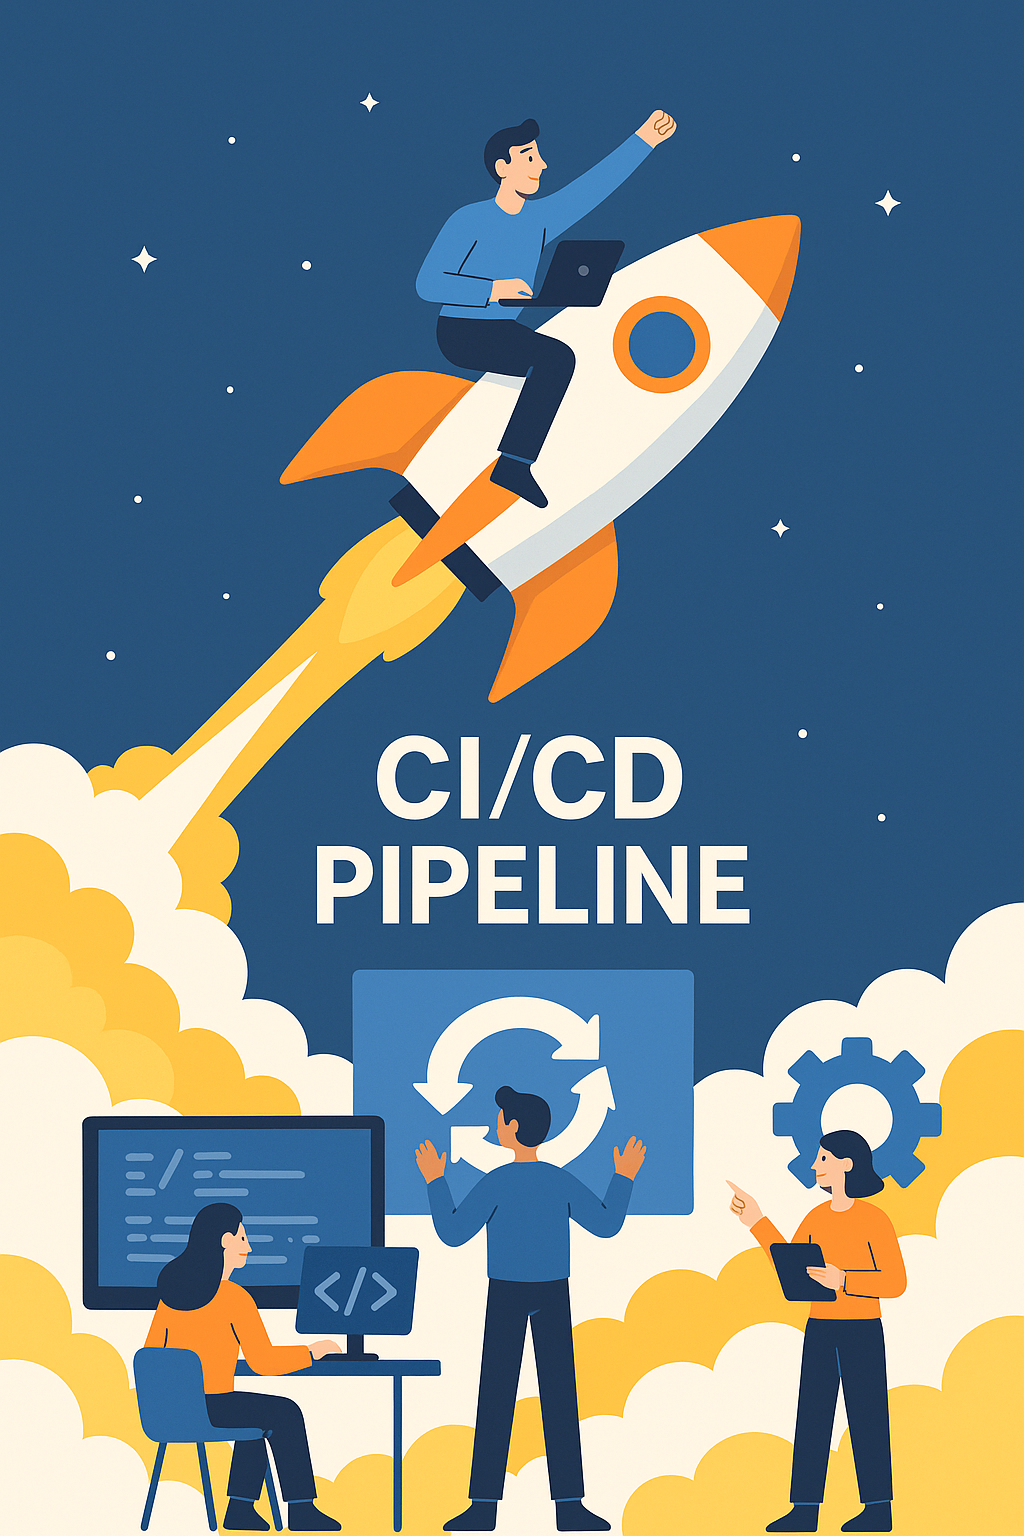
\includegraphics[width=0.5\textwidth]{fig/tothemoon.png}
        \label{fig:ASD-diagram}
    \end{figure}